\documentclass[utf8x, 12pt]{G7-32}

% Настройки стиля ГОСТ 7-32
% Для начала определяем, хотим мы или нет, чтобы рисунки и таблицы нумеровались в пределах раздела, или нам нужна сквозная нумерация.
\EqInChapter % формулы будут нумероваться в пределах раздела
\TableInChapter % таблицы будут нумероваться в пределах раздела
\PicInChapter % рисунки будут нумероваться в пределах раздела
\usepackage{slashbox}

\usepackage[table,xcdraw]{xcolor}

% Добавляем гипертекстовое оглавление в PDF
\usepackage[
bookmarks=true, colorlinks=true, unicode=true,
urlcolor=black,linkcolor=black, anchorcolor=black,
citecolor=black, menucolor=black, filecolor=black,
]{hyperref}

% Изменение начертания шрифта --- после чего выглядит таймсоподобно.
% \usepackage{cyrtimespatched}

% графика
\usepackage{graphicx}
\graphicspath{ {./img/} }

% отделять первую строку раздела абзацным отступом
\usepackage{indentfirst} 

% Пакет Tikz
\usepackage{tikz}
\usetikzlibrary{arrows,positioning,shadows}

% Произвольная нумерация списков.
\usepackage{enumerate}

% ячейки в несколько строчек
\usepackage{multirow}

% itemize внутри tabular
\usepackage{paralist,array}

% объявляем новую команду для переноса строки внутри ячейки таблицы
\newcommand{\specialcell}[2][c]{%
	\begin{tabular}[#1]{@{}c@{}}#2\end{tabular}}

\usepackage{tikz}
\usepackage{pgfplots}
\usepackage{pdfpages}
\usepackage{caption}
\usepackage{longtable}
% \captionsetup[table]{position=top}
% Листинги

\usepackage{listings}
\usepackage{caption}

\usepackage{courier}
\usepackage{wrapfig}

\usepackage{xcolor}
\captionsetup[lstlisting]{singlelinecheck=off, justification=raggedright}


\definecolor{codegreen}{rgb}{0,0.6,0}
\definecolor{codegray}{rgb}{0.5,0.5,0.5}
\definecolor{codepurple}{rgb}{0.58,0,0.82}
\definecolor{backcolour}{rgb}{0.95,0.95,0.92}


% Значения по умолчанию
\lstset{
  % подсветка синтаксиса
  backgroundcolor=\color{backcolour},   
  commentstyle=\color{codegreen},
  keywordstyle=\color{magenta},
  numberstyle=\tiny\color{codegray},
  stringstyle=\color{codepurple},
  basicstyle= \footnotesize,
  breakatwhitespace=true,% разрыв строк только на whitespacce
  breaklines=true,       % переносить длинные строки
%   captionpos=b,          % подписи снизу -- вроде не надо
  inputencoding=koi8-r,
  numbers=left,          % нумерация слева
  numberstyle=\footnotesize,
  showspaces=false,      % показывать пробелы подчеркиваниями -- идиотизм 70-х годов
  showstringspaces=false,
  showtabs=false,        % и табы тоже
  stepnumber=1,
  tabsize=4,              % кому нужны табы по 8 символов?
  frame=single,
  escapeinside={(*}{*)}, %выделение
  literate={а}{{\selectfont\char224}}1
  {б}{{\selectfont\char225}}1
  {в}{{\selectfont\char226}}1
  {г}{{\selectfont\char227}}1
  {д}{{\selectfont\char228}}1
  {е}{{\selectfont\char229}}1
  {ё}{{\"e}}1
  {ж}{{\selectfont\char230}}1
  {з}{{\selectfont\char231}}1
  {и}{{\selectfont\char232}}1
  {й}{{\selectfont\char233}}1
  {к}{{\selectfont\char234}}1
  {л}{{\selectfont\char235}}1
  {м}{{\selectfont\char236}}1
  {н}{{\selectfont\char237}}1
  {о}{{\selectfont\char238}}1
  {п}{{\selectfont\char239}}1
  {р}{{\selectfont\char240}}1
  {с}{{\selectfont\char241}}1
  {т}{{\selectfont\char242}}1
  {у}{{\selectfont\char243}}1
  {ф}{{\selectfont\char244}}1
  {х}{{\selectfont\char245}}1
  {ц}{{\selectfont\char246}}1
  {ч}{{\selectfont\char247}}1
  {ш}{{\selectfont\char248}}1
  {щ}{{\selectfont\char249}}1
  {ъ}{{\selectfont\char250}}1
  {ы}{{\selectfont\char251}}1
  {ь}{{\selectfont\char252}}1
  {э}{{\selectfont\char253}}1
  {ю}{{\selectfont\char254}}1
  {я}{{\selectfont\char255}}1
  {А}{{\selectfont\char192}}1
  {Б}{{\selectfont\char193}}1
  {В}{{\selectfont\char194}}1
  {Г}{{\selectfont\char195}}1
  {Д}{{\selectfont\char196}}1
  {Е}{{\selectfont\char197}}1
  {Ё}{{\"E}}1
  {Ж}{{\selectfont\char198}}1
  {З}{{\selectfont\char199}}1
  {И}{{\selectfont\char200}}1
  {Й}{{\selectfont\char201}}1
  {К}{{\selectfont\char202}}1
  {Л}{{\selectfont\char203}}1
  {М}{{\selectfont\char204}}1
  {Н}{{\selectfont\char205}}1
  {О}{{\selectfont\char206}}1
  {П}{{\selectfont\char207}}1
  {Р}{{\selectfont\char208}}1
  {С}{{\selectfont\char209}}1
  {Т}{{\selectfont\char210}}1
  {У}{{\selectfont\char211}}1
  {Ф}{{\selectfont\char212}}1
  {Х}{{\selectfont\char213}}1
  {Ц}{{\selectfont\char214}}1
  {Ч}{{\selectfont\char215}}1
  {Ш}{{\selectfont\char216}}1
  {Щ}{{\selectfont\char217}}1
  {Ъ}{{\selectfont\char218}}1
  {Ы}{{\selectfont\char219}}1
  {Ь}{{\selectfont\char220}}1
  {Э}{{\selectfont\char221}}1
  {Ю}{{\selectfont\char222}}1
  {Я}{{\selectfont\char223}}1
}

\lstloadlanguages{
  C++
}

% Стиль для псевдокода: строчки обычно короткие, поэтому размер шрифта побольше
\lstdefinestyle{pseudocode}{
  basicstyle=\small,
  keywordstyle=\color{black}\bfseries\underbar,
  language=Pseudocode,
  numberstyle=\footnotesize,
  commentstyle=\footnotesize\it
}

% Стиль для обычного кода: маленький шрифт
\lstdefinestyle{realcode}{
  basicstyle=\scriptsize,
  numberstyle=\footnotesize
}

% Стиль для коротких кусков обычного кода: средний шрифт
\lstdefinestyle{simplecode}{
  basicstyle=\footnotesize,
  numberstyle=\footnotesize
}

% Стиль для BNF
\lstdefinestyle{grammar}{
  basicstyle=\footnotesize,
  numberstyle=\footnotesize,
  stringstyle=\bfseries\ttfamily,
  language=BNF
}

% Определим свой язык для написания псевдокодов на основе Python
\lstdefinelanguage[]{Pseudocode}[]{Python}{
  morekeywords={each,empty,wait,do},% ключевые слова добавлять сюда
  morecomment=[s]{\{}{\}},% комменты {а-ля Pascal} смотрятся нагляднее
  literate=% а сюда добавлять операторы, которые хотите отображать как мат. символы
    {->}{\ensuremath{$\rightarrow$}~}2%
    {<-}{\ensuremath{$\leftarrow$}~}2%
    {:=}{\ensuremath{$\leftarrow$}~}2%
    {<--}{\ensuremath{$\Longleftarrow$}~}2%
}[keywords,comments]

% Свой язык для задания грамматик в BNF
\lstdefinelanguage[]{BNF}[]{}{
  morekeywords={},
  morecomment=[s]{@}{@},
  morestring=[b]",%
  literate=%
    {->}{\ensuremath{$\rightarrow$}~}2%
    {*}{\ensuremath{$^*$}~}2%
    {+}{\ensuremath{$^+$}~}2%
    {|}{\ensuremath{$|$}~}2%
}[keywords,comments,strings]

% Подписи к листингам на русском языке.
\renewcommand\lstlistingname{\cyr\CYRL\cyri\cyrs\cyrt\cyri\cyrn\cyrg}
\renewcommand\lstlistlistingname{\cyr\CYRL\cyri\cyrs\cyrt\cyri\cyrn\cyrg\cyri}



\begin{document}

\frontmatter % выключает нумерацию ВСЕГО; здесь начинаются ненумерованные главы: реферат, введение, глоссарий, сокращения и прочее.
\begin{table}[ht]
	\centering
	\begin{tabular}{|c|p{400pt}|} 
	\hline
		\begin{tabular}[c]{@{}c@{}} 
\includegraphics[scale=0.37]{EmblemBMSTU} \\\end{tabular} &
		\footnotesize\begin{tabular}[c]{@{}c@{}}\textbf{Министерство~науки~и~высшего~образования~Российской~Федерации}\\\textbf{Федеральное~государственное~бюджетное~образовательное~учреждение}\\\textbf{~высшего~образования}\\\textbf{«Московский~государственный~технический~университет}\\\textbf{имени~Н.Э.~Баумана}\\\textbf{(национальный~исследовательский~университет)»}\\\textbf{(МГТУ~им.~Н.Э.~Баумана)}\\\end{tabular}  \\
	\hline
	\end{tabular}
\end{table}
\noindent\rule{\textwidth}{4pt}
\noindent\rule[14pt]{\textwidth}{1pt}
\hfill 
\noindent
\makebox{ФАКУЛЬТЕТ~}%
\makebox[\textwidth][l]{\underline{~~~~«Информатика и системы управления»~~~~~~~~~~~~~~~~~~~~~~~~~~~~~~~~~~~~~~~~~~~~}}%
\\
\noindent
\makebox{КАФЕДРА~}%
\makebox[\textwidth][l]{\underline{~~~~~~~«Программное обеспечение ЭВМ и информационные технологии»~~~~~~~~}}%
\\


\begin{center}
	\vspace{3cm}
	{\bf\huge Отчёт\par}
	{\bf\Large по лабораторной работе №4\par}
	\vspace{0.5cm}
\end{center}


\noindent
\makebox{\large{\bf Название:}~~~}
\makebox[\textwidth][l]{\large\underline{~Параллельный алгоритм трассировки пути~~~~~~~~~~~~~~~~~~~~~~~~}}\\

\noindent
\makebox{\large{\bf Дисциплина:}~~~}
\makebox[\textwidth][l]{\large\underline{~Анализ алгоритмов~~~~~~~~~~~~~~~~~~~~~~~~~~~~~~~~~~~~~~~~~~~~~~~~~~~~}}\\

\vspace{1.5cm}
\noindent
\begin{tabular}{l c c c c c}
    Студент      & ~ИУ7-55Б~               & \hspace{3.5cm} & \hspace{3.5cm}                 & &  И. Е. Афимин \\\cline{2-2}\cline{4-4} \cline{6-6} 
    \hspace{3cm} & {\footnotesize(Группа)} &                & {\footnotesize(Подпись, дата)} & & {\footnotesize(И.О. Фамилия)}
\end{tabular}

\vspace{1cm}

\noindent
\begin{tabular}{l c c c c}
    Преподаватель & \hspace{6cm}   & \hspace{3.5cm}                 & & Л.Л. Волкова \\\cline{3-3} \cline{5-5} 
    \hspace{3cm}  &                & {\footnotesize(Подпись, дата)} & & {\footnotesize(И.О. Фамилия)}
\end{tabular}

\begin{center}	
	\vfill
	\large \textit {Москва, 2020}
\end{center}

\thispagestyle {empty}
\pagebreak

\tableofcontents

\newpage
\Introduction    
Трассировка лучей  — один из методов геометрической оптики — исследование оптических систем путём отслеживания взаимодействия отдельных лучей с поверхностями. Трассировка пути  — методика рендеринга в компьютерной графике, которая стремится симулировать физическое поведения света настолько близко к реальному, насколько это возможно.

    Целью данной лабораторной работы является изучение и реализация параллельных вычислений
    для обратного трассировщика лучей.

    Задачи данной лабораторной работы:
    \begin{enumerate}
        \item изучить алгоритм обратной трассировки лучей;
        \item реализовать алгоритм обратной трассировки лучей;
        \item провести замеры процессорного времени работы от разного числа параллельных потоков;
        \item провести сравнение параллельных реализаций алгоритма обратной трассировки лучей со стандартной реализацией.
    \end{enumerate}

\newpage

\mainmatter % это включает нумерацию глав и секций в документе ниже
\chapter{ Аналитический раздел}
\label{cha:analytical}
    В данном разделе будут рассмотрены основные теоритические понятия алгоритма трассировки пути.

    \section{Алгоритм трассировки пути}
	Методы трассировки лучей на сегодняшний день считаются наиболее мощными методами создания реалистических изображений. Универсальность методов трассировки в значительной степени обусловлена тем, что в их основе лежат простые и ясные понятия, отражающие опыт восприятия окружающего мира.

	Метод трассировки пути позволяет значительно сократить перебор световых лучей по сравнению с классической трассировкой. В нем отслеживаются лучи не от источников, а из камеры. Таким образом, трассируется определенное число лучей, равное разрешению картинки.

	Предположим, что у нас есть камера и экран, находящийся на расстоянии d от нее (рисунок \ref{png:axis}).

        \begin{figure}[h!]
            \centering
            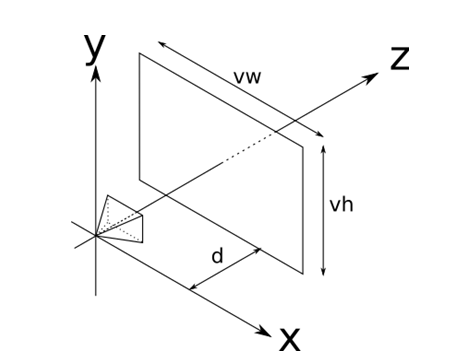
\includegraphics[scale=0.6]{axis.png}
	 \caption{Расположение камеры и сцены}
            \label{png:axis}
        \end{figure} 

 Разобьем экран на квадратики. Дальше будем по очереди проводить лучи из камеры в центр каждого квадратика (первичные лучи). Найдем пересечение каждого такого луча с объектами сцены и выберем среди всех пересечений самое близкое к камере. Далее, применив нужную модель освещения, можно получить изображение сцены.

	Но можно пойти дальше. Если мы хотим смоделировать такое явление, как отражение, нам необходимо из самого близкого пересечения пустить вторичные лучи. Например, если поверхность отражает свет и она идеально ровная, то необходимо отразить первичный луч от поверхности и пустить по этому направлению вторичный луч.

	Исходя из того, как работает данный алгоритм, можно сделать вывод о том, что выпускать лучи для каждого пиксела можно независимо друг от друга. Поэтому данную часть алгоритма целесообразно выполнять параллельно.

\section{Вывод}
Был рассмотрен алгоритм трассировки пути и сделан вывод о том, что данный алгоритм является лучшим для визуализации реалистичного изображения. Так же рассмотрен вариант распараллеливания алгоритма.


\chapter{ Констукторский раздел}
\label{cha:design}
    В данном разделе будет рассмотрена схема алгоритма, требования к функциональности ПО,
    и опредены способы тестирования.
    
    \section{Разработка алгоритма}
        Ниже будет представлена схема алгоритма трассировки пути.

        Алгоритм трассировки пути (рисунок \ref{schema:rtx});


    \begin{figure}[h!]
        \centering
            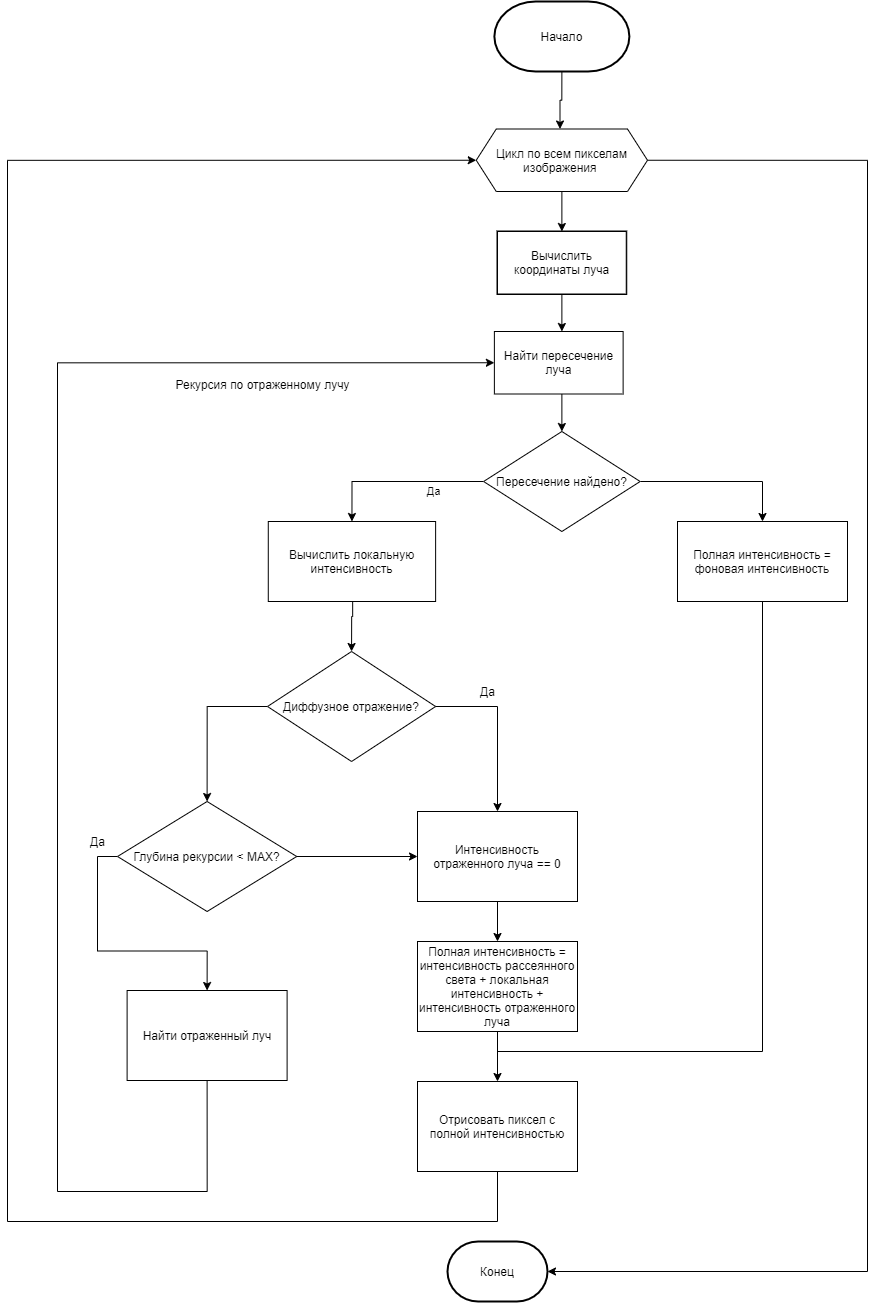
\includegraphics[scale=0.5]{rtx.png}
            \caption{Схема алгоритма трассировки пути}
            \label{schema:rtx}
    \end{figure}

    \section{Параллельные вычисления}
Распрараллеливание программы должно уменьшать время работы. Это достигается за счет выполнения параллельно участков кода (например, в циклах с большим количеством независимых вычилений).

В предложенном алгоритме данным участком будет являться основной двойной цикл вычислений.
Данный блок программы как раз предлагается распараллелить.


    \section{Требования к функциональности ПО}
        В данной работе требуется обеспечить следующую минимальную функциональность оконного приложения:
        \begin{enumerate}
	\item обеспечить ввод количества потоков;
            \item обеспечить возможность просмотра полученного с помощью алгоритма трассировки пути изображения;
            \item обеспечить вывод замеров времени работы алгоритма трассировки пути.
        \end{enumerate}

    \section{Методы тестирования}
    Тестирование ПО будет проводиться методом черного ящика.

\section{Вывод}
В данном разделе рассмотрена схема алгоритма трассировки пути и конкретизирован способ распараллеливания алгоритма.


\chapter{ Технологический раздел}
\label{cha:technological}

    В данном разделе будут выбраны средства реализации ПО и представлен листинг кода. 


    \section{Средства реализации}
        Для реализации программ я выбрал язык программирования C++, так как имею большой опыт работы с ним.
	Для замера процессорного времени была использована стандартная библиотека C++ - chrono \cite{link_time}.
        В качестве среды разработки использовался CLion 2020 \cite{link4}.

	Для распараллеливания были использованы потоки стандартной библиотеки C++ \cite{link5}.


        \begin{lstlisting}[label=lst:rtx_parall, caption=Реализация алгоритма трассировки пути с параллельными вычислениями]
    int n = 8; // Количество потоков

    int step = image_width / n;

    std::vector<std::thread *> threadArr;

    int x1 = 0;
    int x2 = step;

    int y1 = 0;
    int y2 = image_height;

    auto buf = new color_buf[image_width * image_height];
    for (int i = 0; i < image_width * image_height; i++)
    {
        buf[i].x1 = 0;
        buf[i].x2 = 0;
        buf[i].x3 = 0;
    }

    for (int i = 0; i < n; i++)
    {
        auto* newThread = new std::thread(cycle, x1, y2, x2, y1, samples_per_pixel, cam, background, world, max_depth, image_width, image_height, buf);
        
		threadArr.push_back(newThread);

        x1 = x2;
        x2 += step;
    }

    for (int i = 0; i < n; i++)
    {
        threadArr[i]->join();
    }

    std::ofstream out;
    out.open("img228.ppm");
    out << "P3\n" << image_width << ' ' << image_height << "\n255\n";

    for (int i = 0; i < 90000; i++)
    {
        out << buf[i].x1 << ' ' << buf[i].x2 << ' ' << buf[i].x3 << "\n";
    }
        \end{lstlisting}


\section{Вывод}
В данном разделе была рассмотрены средства реализации алгоритма и представлена реализация алгоритма трассировки пути.


\chapter{Экспериментальный раздел}
\label{cha:research}
    В данном разделе будут выполнены эксперименты для проведения 
    сравнительного анализа алгоритма трассировки пути по затрачиваемому процессорному 
    времени в зависимости от числа потоков.

    \section{Сравнительный анализ на основе замеров времени работы алгоритмов}
	 В рамках данного проекта был произведен замер времени работы алгоритма обратной трассировки лучей при количестве потоков равном 1, 2, 4, 8, 16, 32, 64.
	Результаты данных измерений приведены на графике \ref{graph:1}.

        Тестирование проводилось на ноутбуке с процессором
        Intel(R) Core(TM) i5-8250U CPU, 8 логических процессоров,
        под управлением Windows 10 с 8 Гб оперативной памяти.

    \begin{figure}[h!]
        \centering
        \begin{tikzpicture}
            \begin{axis}[
                legend pos = north west,
                grid = major,
                xlabel = Число потоков,
                ylabel = {Время, секунды},
                height = 0.5\paperheight, 
                width = 0.75\paperwidth
            ]
            
            \addplot table[x=n,y=time] {data/workTime.dat};
            \end{axis}
        \end{tikzpicture}
        \caption{График зависимости времени работы алгоритма трассировки пути от числа потоков} 
        \label{graph:1}
    \end{figure}


\section{Вывод}
        В ходе экспериментов по замеру времени работы было установлено:
	\begin{enumerate}
	\item параллельная реализация алгоритма трассировки пути в случае увеличения числа потоков в 2 раза, начиная с 8 замедляет скорость своей работы;
	\item максимальный прирост скорости параллельной реализации алгоритма трассировки пути достигается при количестве потоков равных 8 и равен  $ \approx 5.32 $ раза.

        \end{enumerate}


\Conclusion
    В ходе выполнения лабораторной работы были выполнены следующие задачи:
    \begin{enumerate}
        \item изучен алгоритм параллельной трассировки пути;
        \item реализован алгоритм параллельной трассировки пути;
        \item проведены замеры процессорного времени работы от разного числа параллельных потоков;
        \item проведено сравнение параллельных реализаций алгоритма трассировки пути со стандартной реализацией.
    \end{enumerate}

В ходе сравнения процессорного времени работы было установлено:
	\begin{enumerate}
	\item параллельная реализация алгоритма трассировки пути в случае увеличения числа потоков в 2 раза, начиная с 8 замедляет скорость своей работы;
	\item максимальный прирост скорости параллельной реализации алгоритма трассировки пути достигается при количестве потоков равных 8 и равен  $ \approx 5.32 $ раза.

        \end{enumerate}


Эксперементальным путем было выяснено, что увеличение количества потоков в 2 раза не всегда увеличивает производительность программы.

    
 
%далее сам список используевой литературы
\begin{thebibliography}{}
    \bibitem{link_time}  Date and time utilities. // [Электронный ресурс]. Режим доступа: https://en.cppreference.com/w/cpp/chrono, (дата обращения: 20.10.2020).
    \bibitem{link2}  C/C++: как измерять процессорное время. // [Электронный ресурс]. Режим доступа: https://habr.com/ru/post/282301/, (дата обращения: 20.10.2020).
    \bibitem{link3}  Path tracing. // [Электронный ресурс]. Режим доступа: $https://en.wikipedia.org/wiki/Path_tracing$, (дата обращения: 20.10.2020).
    \bibitem{link4}  Clion. // [Электронный ресурс]. Режим доступа: $https://www.jetbrains.com/clion/$, (дата обращения: 20.10.2020).
    \bibitem{link5}  std::thread. // [Электронный ресурс]. Режим доступа: $https://en.cppreference.com/w/cpp/thread/thread$, (дата обращения: 20.10.2020).
\end{thebibliography}

\end{document}